\documentclass[class=scrbook, crop=false]{standalone}
\usepackage[subpreambles=true]{standalone}
\ifstandalone
    % WARNING: Proceed with caution!

% -----------------------------------------------------------------------------------
% For package standalone
% -----------------------------------------------------------------------------------
\usepackage{import}

% -----------------------------------------------------------------------------------
% Language and typeset
% -----------------------------------------------------------------------------------
\usepackage[ngerman, english]{babel}

\usepackage{subcaption}
% Umlauts and other special characters (UTF-8)
% \usepackage[utf8]{inputenc}
\usepackage{fontspec}
\setsansfont{Arial}
% \usepackage[T1]{fontenc}  % Enable accented characters and umlauts
% LuaLatex doesn't need fontenc and uses UTF-8
% \usepackage{lmodern}  % Font face


% --------------------------------------------------------------------------------
% Page formatting
% --------------------------------------------------------------------------------
% Change the header/footer for chapter beginnings and normal pages
\usepackage[automark,headsepline]{scrlayer-scrpage}

% The package provides an easy and flexible user interface to customize the page
% layout, implementing auto-centering and auto-balancing mechanisms
% WARNING: WHEN CHANGING BCOR (Binding correction), the cover needs reworking!...
\newcommand{\theBCOR}{15mm}  % Define binding correction
\usepackage[
    bindingoffset=\theBCOR,
    % showframe, % Show boxes which indicate margins and paddings
    bottom = 3.5cm, % Margins
      left = 2.5cm,
     right = 2.5cm
] {geometry}

% The package 'float' provides a container for document objects which can not be
% broken over pages, such as tables and figures
% Needed for table and figure indexes  
\usepackage{float}

% support for landscape layout
\usepackage{lscape}

% support of \tablenotes command to add notes under table
\usepackage{threeparttable}

% To allow drawing more professional tables
\usepackage{booktabs}

% --------------------------------------------------------------------------------
% Contents
% --------------------------------------------------------------------------------
% Vector graphics (for Cover page)
\usepackage{tikz} 

% Allows additional parameters when including images
\usepackage{graphicx}

% Roman font family for all headings
\addtokomafont{disposition}{\rmfamily}

% Set the line spacing to 1.5
\usepackage[onehalfspacing]{setspace}

% Improves overall text spacing
% http://www.khirevich.com/latex/microtype/
\usepackage[stretch=10]{microtype}

% Math symbols like mu outside the math environment
\usepackage{textcomp}

% A comprehensive (SI) units package∗
% For defining SI units
\usepackage[
    range-units=single,         % Formatting ranges with single unit indication: 1 - 2 m
    range-phrase=-,             % Phrase for range: 1 - 2 m vs 1 to 2 m
    separate-uncertainty=true,  % sets +- between value and uncertainty 
    multi-part-units=repeat     % In expressions with multiple values (multi part numbers) 
                                % the unit is printed each time: 1 mm x 1 mm
] {siunitx}
% https://tex.stackexchange.com/questions/124488/multi-part-numbers-and-units-in-siunitx

% Allows Sourcecodes with highlighting 
\usepackage{listings}

% This package provides user control over the layout of the three basic list
% environments: enumerate, itemize and description
\usepackage{enumitem}
\setlist{nosep} % Remove the vertical space between \item elements in all lists

% ToDo Notes
% \setlength{\marginparwidth}{2cm}
\usepackage{todonotes}
\setuptodonotes{inline, inlinepar}
\reversemarginpar  % Put ToDo notes on the binding's side
% \usepackage{soul} % Colorful ToDo notes

% Check out colors here http://latexcolor.com/
\usepackage{xcolor}

\usepackage{amsmath}    % alignment of equations

% --------------------------------------------------------------------------------
% Other elements
% --------------------------------------------------------------------------------
% Blindtext: Organic looking text dummy
\usepackage{blindtext}

% Hyperlinks within the document (PDF)
% "hidelinks" hides visual highlighting of links
\usepackage[hidelinks]{hyperref}

% Package for Glossary and Index (Acronyms are listed in a separate list) 
\usepackage[acronym, nogroupskip]{glossaries}[=v4.49] % groupskip: alphabetic grouping of entries

\usepackage{xltabular}   % <------- FOR glossaries

% Integration and management of bibliographies
\usepackage{csquotes}   % backend=biber in biblatex needs this package
\usepackage[
    style=ieee,   % style of the bibliography, entries are sorted in alphabetic order. "ieee" is another common style.
    backend=biber,      % based on package 'biber' 
    bibencoding=ascii   % ASCII Text encoding; may use "utf8" instead
] {biblatex}

% --------------------------------------------------------------------------------
%                               PATHS & FILES
% --------------------------------------------------------------------------------
% Fix paths for standalone compiling
\ifstandalone
    \def \home {..}
\else
    \def \home {.}
\fi

% Package: scrlayer-scrpage
% \def \stylePath {\home/settings+/style/page}
\input{\home/settings+/style/page}  % Load page style

% Package: graphicx
\graphicspath{{\home/images/}}  % Set path to images

% Package: listings
\input{\home/settings+/style/code.tex}  % Set path to style file
\lstset{inputpath={\home/code/}} % Default path to code listings

% Package: glossaries
\input{\home/settings+/style/symbols}  % Set path to symbols list style file
\input{\home/settings+/style/acronyms}  % Set path to acronym list style file
% -------------------------------------------------------------------------------
%               Listing of all Glossary and Acronym Entries 
%                           use as shown below
% -------------------------------------------------------------------------------

% ==== EXEMPLARY ENTRY FOR SYMBOLS LIST =========================================

% ==== EXEMPLARY ENTRY FOR ACRONYMS LIST ========================================
% \newacronym{#label}{#acronym}{#long_form}

% define new command for custom arconym entry with only two arguments
% fabricates an easier way to use \newacronym 
\newcommand{\acroX}[2]{\newacronym{#1}{#1}{#2}}
% \acroX{label and arconym}{long name}
% \acroX{CD}               {Compact Disk}

\newcommand{\acroY}[3]{\newacronym{#1}{#2}{#3}}
% \arcoY{label}{acronym}{long name}
% \acroY{CD}   {cd}     {Compact Disk}
 
\newacronym{AEP}{AEP}{Imbalance price}
\newacronym{aFRR}{aFRR}{Automatic Frequency Restoration Reserve}


\newacronym{reBAP}{reBAP}{Uniform imbalance price}
\newacronym{TSO}{TSO}{Transmission System Operator}
\newacronym{FCR}{FCR}{Frequency Containment Reserve}
\newacronym{mFRR}{mFRR}{Manual Frequency Restoration Reserve}
\newacronym{BRP}{BRP}{Balancing Responsible Party}
\newacronym{SB}{SB}{System Balance}
\newacronym{VRE}{VRE}{variable renewable energy}
\newacronym{ID1}{ID1}{intraday index ID1}
\newacronym{MAE}{MAE}{mean average error}
\newacronym{RMSE}{RMSE}{root mean squared error}
\newacronym{MSE}{MSE}{mean squared error}
\newacronym{CRPS}{CRPS}{continuous ranked probabililty score}
\newacronym{GCC}{GCC}{Grid Control Cooperation}
\newacronym{IC}{IC}{Continuous intraday}
\newacronym{VWAP}{VWAP}{volume-weighted average price}
\newacronym{VID}{VID}{traded volume within the intraday market}
\newacronym{ID AEP}{ID AEP}{Intraday Average Energy Price}
\newacronym{FRR}{FRR}{Frequency Restoration Reserve}
\newacronym{TFT}{TFT}{Temporal Fusion Transformer}
\newacronym{DLM}{DLM}{Dynamic Linear Model}
\newacronym{GB}{GB}{Gradient Boosting}
\newacronym{RF}{RF}{Random Forest}
\newacronym{ARIMAX}{ARIMAX}{Autoregressive Integrated Moving Average with eXogenous variables}
\newacronym{xLSTM}{xLSTM}{Extended Long Short-Term Memory}
\newacronym{DWD}{DWD}{Deutscher Wetterdienst}
\newacronym{ENTSO-E}{ENTSO-E}{European Network of Transmission System Operators for Electricity}
\newacronym{IDA1}{IDA1}{Intraday auction 1}
\newacronym{MOSMIX}{MOSMIX}{Model Output Statistics-MIX}
\newacronym{mLSTM}{mLSTM}{memory-optimized LSTM}
\newacronym{sLSTM}{sLSTM}{speed-optimized LSTM}

% ==== EXEMPLARY ENTRY FOR MAIN GLOSSARY ========================================

    % \newglossaryentry{policy}{name={Policy},description={Im geschäftlichen Bereich bezeichnet Policy eine interne Leit- bzw. Richtlinie, die formal durch das Unternehmen dokumentiert und über ihr Management verantwortet wird}}
    % \newglossaryentry{pcie}{name={PCI Express},description={PCI Express („Peripheral Component Interconnect Express“, abgekürzt PCIe oder PCI-E) ist ein Standard zur Verbindung von Peripheriegeräten mit dem Chipsatz eines Hauptprozessors. PCIe ist der Nachfolger von PCI, PCI-X und AGP und bietet im Vergleich zu seinen Vorgängern eine höhere Datenübertragungsrate pro Pin.}}
    % \newglossaryentry{realnumber}
  % Load glossary, symbol and acronyms list

% Package: biblatex
\addbibresource{\home/references/references.bib}  % Set path to bib resources

% Custom variables
\input{\home/settings+/variables}
% --------------------------------------------------------------------------------
%                                   OPTIONAL
% --------------------------------------------------------------------------------


% Simple arithmetic for LaTeX commands
% \usepackage{calc}

% Document Elements
% -------------------

% Index
% \usepackage{imakeidx}

% compact Lists
%\usepackage{paralist}

% visual improvements for citations
% \usepackage{epigraph}

% Create pseudo code
% https://www.overleaf.com/learn/latex/Algorithms
% \usepackage{algorithm}
% \usepackage{algorithmic}
%\usepackage[noend]{algpseudocode}

% Formatting
% -------------------
% Tweaks for scrbook, redefines commands of other packages
% \usepackage{scrhack}

% Intelligent space separator (nice for superscript?)
% \usepackage{xspace}

% Allows breaks within tables
%\usepackage{tabularx}

% Allows for page breaks in tables
% \usepackage{longtable}

% allows modifying of captions
% \usepackage{caption}

% Multiline comments
%\usepackage{verbatim}

% % Custom colors
% \definecolor{dartmouthgreen}{rgb}{0.05, 0.5, 0.06}

% IF you want to define unicode characters
% \DeclareUnicodeCharacter{0229}{\c{e}}
% \DeclareUnicodeCharacter{0306}{\u{Z}}


% Document elements
% ------------------------------------

% Table package
% \usepackage{booktabs}

% Pie diagram
% \usepackage{datapie}

% Side by Side images
% \usepackage{subcaption}

% For landscape tables
%\usepackage{pdflscape}
%\usepackage{afterpage}

% Graphics can be flow around by text
%\usepackage{wrapfig}

\fi

% ----------------------------------------------------------------------------
%                               State of the Art
% ----------------------------------------------------------------------------
\begin{document}

\chapter{State of the Art}
\label{Chapter::State_of_the_Art} % Outline text
This chapter reviews relevant literature in two major areas: first, studies focused on forecasting imbalance prices in electricity markets; and second, general advances in time series forecasting models. 
By distinguishing between market-specific forecasting objectives (e.g., price vs. volume, national market rules) and model-centric developments (e.g., deep learning architectures), the chapter provides a structured overview of the current state of the art.
 It concludes by positioning the present thesis within this research landscape and outlining its contributions in terms of methodological innovation and application domain.
%In this chapter models and papers for the prediction of the german imbalance price as well as general time series predictors will be discussed. 
%This chapter will conclude by showing how this thesis fits into the current ecosystem.
%With this information I will conclude this chapter by showing how this thesis fits into the current ecosystem.

% Topics that are similar to yours but are already published.
% Explain their approach and what the difference to your approach is.
\section{Related Work}
\label{Section::Related_Work}
Several studies have addressed forecasting tasks on European imbalance markets. Most of this research has focused on the British energy market, where the settlement period differs from Germany, typically spanning 30 minutes instead of 15 \cite{narajewskiProbabilisticForecastingGerman2022} \cite{limaBayesianPredictiveDistributions2023}. Table \ref{Table::Related_Work} shows an overview about related works on this topic. The contents of the table are explained further in the following paragraphs.

A subset of these studies targets imbalance volume forecasting. For instance, García and Kirschen \cite{garciaForecastingSystemImbalance2006} applied ARIMA, exponential smoothing, and caterpillar forecasting to predict total imbalance volume in the UK. Similarly, works on the Belgian \cite{bottieauVeryShortTermProbabilisticForecasting2020} \cite{dumasProbabilisticForecastingImbalance2019} and Hungarian  \cite{balazsShorttermSystemImbalance2024} markets primarily focus on volume prediction, employing statistical and machine learning methods.

In contrast, other studies focus on imbalance price prediction. Lima et al. \cite{limaBayesianPredictiveDistributions2023} proposed a Dynamic Linear Model (DLM) and demonstrated its superiority over GARCH and AR-GARCH models. They identified net imbalance volume and scarcity metrics as key predictive features. Ganesh and Bunn  \cite{ganeshForecastingImbalancePrice2024} compared various deep learning models, including RNNs, LSTMs, GRUs, FCNNs, TFT, and N-BEATS. Their findings indicated that even simple FCNNs outperformed classical models such as DLM.

Several works emphasize the effect of forecast lead time. For instance, Browell and Gilbert \cite{browellPredictingElectricityImbalance2022} found that prediction accuracy improves substantially as the forecast horizon shortens. Their approach combined kernel density estimation and linear regression to model UK imbalance prices.

More recently, advanced deep learning methods have been explored. Deng et al. \cite{dengSeasonalityDeepLearning2024} introduced BiLSTM and SA-BiLSTM architectures, showing performance gains for multi-step forecasting tasks. Lucas et al. \cite{lucasPriceForecastingBalancing2020} applied gradient boosting (GB), random forests (RF), and XGBoost to UK imbalance prices, finding RF to perform best. These studies consistently identified net imbalance volume as the most important input feature.

In the German market, research remains sparse. Narajewski \cite{narajewskiProbabilisticForecastingGerman2022} used probabilistic models, including LASSO regression, GAMLSS, and probabilistic neural networks (PNN), to predict the reBAP. Their approach involved dataset stratification and model specialization for different data segments.

Notably, many UK-based models were trained on pre-COVID data, potentially limiting their relevance for today’s market dynamics  \cite{abadieEnergyMarketPrices2021}. Moreover, few studies consider high-frequency imbalance settlement (15-minute granularity) or the specific German reBAP calculation with its modular pricing mechanism.

This thesis contributes to the field by:
\begin{itemize}
\item focusing on the German imbalance price (reBAP) with quarter-hourly resolution
\item comparing established methods (RF, ARIMA) with novel time series architectures (xLSTM, iTransformer)
\item incorporating a broader set of operational and meteorological input features from ENTSO-E, Netztransparenz, and DWD
\end{itemize}

\begin{table}

    \centering
\begin{tabular}{l|l|l|l|l}
Paper & Market & Target & Models used & Time resolution  \\\hline
Lima et al.  \cite{limaBayesianPredictiveDistributions2023}	&UK	&Price	&DLM, GARCH, AR-GARCH	&30 min	 \\
Ganesh \& Bunn  \cite{ganeshForecastingImbalancePrice2024}	 &UK&Price	&FCNN, LSTM, GRU, TFT, N-BEATS&	30 min	 \\
Garcia \& Kirschen  \cite{garciaForecastingSystemImbalance2006}	&UK	&Volume&	ARIMA, exponential smoothing&	30 min	 \\
Browell \& Gilbert \cite{browellPredictingElectricityImbalance2022}&	UK&	Price	&KDE, linear regression	&30 min	 \\
Lucas et al.  \cite{lucasPriceForecastingBalancing2020}&UK&	Price	&RF, XGBoost, GB	&30 min	 \\
Deng et al.  \cite{dengSeasonalityDeepLearning2024}	&UK	& Price	&BiLSTM, SA-BiLSTM&	30 min \\
Narajewski \cite{narajewskiProbabilisticForecastingGerman2022}&Germany&	Price	&LASSO, GAMLSS, PNN	&15 min	 \\
Bottieau et al.  \cite{bottieauVeryShortTermProbabilisticForecasting2020}&	Belgium	&Volume&Prob. Forecasting (2-Step)	&15 min	\\
Balázs et al. \cite{balazsShorttermSystemImbalance2024}	&Hungary&	Volume	&Linear/Non-linear models&	15 min \\
This work	&Germany&	 Price&	xLSTM, iTransformer, RF, ARIMA	&15 min\\
\end{tabular}
\caption{Overview about related work}
\label{Table::Related_Work}
\end{table}

%Several other papers have worked on forecasting on the imbalance market. Different energy markets are structured differently. While the imbalance is settled every quarter hour in germany \cite{narajewskiProbabilisticForecastingGerman2022}, each settlement period is 30 minutes on the energy market in the united kingdom \cite{limaBayesianPredictiveDistributions2023}.


%The works \cite{limaBayesianPredictiveDistributions2023} \cite{ganeshForecastingImbalancePrice2024} \cite{garciaForecastingSystemImbalance2006} \cite{browellPredictingElectricityImbalance2022} \cite{lucasPriceForecastingBalancing2020} \cite{dengSeasonalityDeepLearning2024} focus on the energy market in the united kingdom and use different approaches. While \cite{limaBayesianPredictiveDistributions2023}, \cite{ganeshForecastingImbalancePrice2024}, \cite{browellPredictingElectricityImbalance2022}, \cite{lucasPriceForecastingBalancing2020} and \cite{dengSeasonalityDeepLearning2024} try to make a prediction about the imbalance price, \cite{garciaForecastingSystemImbalance2006} tries to forecast the total imbalance volume. 

%The volume is forecasted using three different methods, ARIMA, exponential smoothing and caterpillar forecasting.

%For the papers predicting imbalance prices different models where used.
%The authors of \cite{limaBayesianPredictiveDistributions2023} developped a dynamic linear model (DLM) and compared their results to GARCH and AR-GARCH. Their model outperformed GARCH and AR-GARCH on all their out-of-sample forecasting experiments. During their research they also inspected how the imbalance price correlates with the features used in their predictions.
%The net imbalance volume was the features with the largest correlation, followed by metrics which try to capture the scarcity of energy.
%In \cite{ganeshForecastingImbalancePrice2024} many different neural network algorithms were compared, namely Recurrent Neural Networks (RNN), Long Short Term Memory (LSTM), Gated Recurrent Units (GRU), Temporal Fusion Transformer (TFT), Fully Connected Neural Networks (FCNN) and the Neural basis expansion analysis for interpretable time series forecasting (N-BEATS). The FCNNs used in this paper were a significant improvement to the DLM developed in \cite{limaBayesianPredictiveDistributions2023}.
%The authors of \cite{browellPredictingElectricityImbalance2022} investigated how much impact the prediction time has on the result. They used Kernel Density Estimators (KDE) and linear regression to get a forecast for the imbalance price. Another result was, that the prediction quality greatly improves if the prediction is done at a time closer to delivery time.
 
% For the imbalance price prediction \ref{lucasPriceForecastingBalancing2020} employed Gradient Boosting (GB), Random Forest (RF) and XGBoost. Out of the models they used RF performed the best. During their research they also looked into feature importance for all their models. They found that the net imbalance volume was the most important feature.
 
% In \cite{dengSeasonalityDeepLearning2024} a new Bidirectional LSTM (BiLSTM) and Seasonal Attention BiLSTM (SA-BiLSTM) were compared to the previously used models. The authors looked into forecasting for multiple settlement periods into the future, with SA-BiLSTM performing the best in most of the cases.
 
%Apart from the UK energy market some research on the Belgian \cite{bottieauVeryShortTermProbabilisticForecasting2020} \cite{dumasProbabilisticForecastingImbalance2019}, Hungarian \cite{balazsShorttermSystemImbalance2024} and German \cite{narajewskiProbabilisticForecastingGerman2022} electricity market was published.
%In the papers \cite{bottieauVeryShortTermProbabilisticForecasting2020} and \cite{balazsShorttermSystemImbalance2024} the authors used machine learning methods and auto regressive methods to predict the system imbalance in their respective energy market.
%A two step probabilistic approach was suggested in \cite{dumasProbabilisticForecastingImbalance2019}. First the system imbalance is forecasted and this information is then used in a second prediction for the imbalance price.

%The paper on the german electricity market \cite{narajewskiProbabilisticForecastingGerman2022} used lasso regression, gamlss and a probabilistic neural network (PNN) to try to predict the imbalance price for the german electricity market. The data for their models was split into subsets and different models with different hyperparameter configurations trained for each subset.

%Many of the mentioned papers, especially the ones on the british electricity market used data from before the COVID-19 pandemic. During the pandemic the energy market changed. Models based and calibrated on pre-pandemic data can not be used to effectively forecast current energy prices \cite{abadieEnergyMarketPrices2021}.


%In this thesis different models are compared on the task of predicting the imbalance price. 
%For this task random forest, arimax, xLSTM (an extension of LSTM) \cite{beckXLSTMExtendedLong2024} and a new inverted Transformer (iTransformer) \cite{liuITransformerInvertedTransformers2023} architecture will be inspected.
%Random forest performed well on the task of predicting the imbalance price before the COVID-19 pandemic \ref{lucasPriceForecastingBalancing2020}.


\section{Time Series Predictors}
\label{Section::Time_Series_Predictors}
Recent years have seen substantial advances in deep learning-based time series forecasting. In this thesis, two promising architectures are investigated: xLSTM, an enhanced recurrent model based on LSTM, and iTransformer, a Transformer variant tailored for multivariate time series.

Both models aim to address typical challenges in energy market forecasting, such as irregular patterns, long-term dependencies, and variable importance across different input features.

The following subsections outline the underlying concepts and innovations of these architectures.

%In this thesis established machine learning models are compared with novel approaches for Time Series Predictors. These newer models will be introduced in the next two subsections.

%\subsection{ARIMA}
%\label{Section::ARIMA}

%\subsection{Random Forest}
%\label{Section::Random_Forest}


\subsection{xLSTM}
\label{Section::xLSTM}
xLSTM (Extended Long Short-Term Memory) is an architecture that builds upon the classical LSTM framework to match the performance of Transformer models while preserving the low computational complexity of recurrent networks [20]. The architecture introduces two novel types of memory cells: sLSTM and mLSTM, each designed to increase expressiveness and flexibility in sequence modeling.
\begin{itemize}
\item \textit{sLSTM} modifies the standard gating mechanism by replacing the input gate's sigmoid activation with an exponential function. This allows for stronger input modulation. The forget gate may use either sigmoid or exponential activation. sLSTM also enables memory mixing via multiple memory channels with recurrent connections.
\item \textit{mLSTM} extends the traditional LSTM by using a matrix-valued memory instead of a single vector. This allows the model to capture richer temporal patterns. While mLSTM does not support memory mixing, it can also use exponential gating and benefit from deeper memory representations.
\end{itemize}

Both variants can be embedded in residual blocks, enabling dimension transformation and stable gradient propagation. A typical xLSTM stack consists of interleaved sLSTM and mLSTM layers, allowing a trade-off between model depth and capacity.

The main advantage of xLSTM is its linear time complexity and constant memory footprint with respect to sequence length, which is particularly useful in high-resolution datasets such as 15-minute reBAP time series.


%Extended Long Short-Term Memory (xLSTM) is a novel model which is based on the existing Long Short-Term Memory (LSTM) \cite{gravesLongShortTermMemory2012}. The recent advances in Transformer technology outperformed LSTM models. 
%The goal behind the development of xLSTM was to check whether LSTM models could reach comparable results if the models use the same amount of parameters.
%xLSTM introduces two new LSTM cells, sLSTM and mLSTM.

%In the sLSTM Cell the activation function is changed. While in LSTM the activation function for the input gate is the sigmoid function, sLSTM uses the exponential function. In sLSTM the activation for the forget gate can be either the sigmoid function or the exponential function. sLSTM cells can also have multiple memory cells. This enables memory mixing via recurrent connections. A residual sLSTM cell contains a sLSTM  cell which summarizes the past in the original space. This is then linearly mapped into a higher-dimensional  space where the non linear activation function is applied. Afterwards the result is mapped back to the original space.

%The second alteration of the basic LSTM cell uses a matrix memory instead of a single value. This cell is called mLSTM. It also uses exponential gating for the input gate and either sigmoid or exponential gating for the forget gate. This cell can also have multiple memorry cells, but does not support memory mixing. In a residual mLSTM cell a pre-projection linearly maps to a high-dimensional space. The mLSTM cell then summarizes the past in the high dimensional space. The result is then linearly mapped back to the original space.

%An xLSTM architecture is constructed by stacking theses building blocks. An advantage of xLSTM networks is, that the computation complexity is linear and the memory complexity is constant with respect to sequence length. \cite{beckXLSTMExtendedLong2024}



\subsection{iTransformer}
\label{Section::iTransformer}

Transformers have become a standard in time series forecasting, but their performance often degrades on multivariate inputs with many variables and relatively short sequence lengths — a common situation in energy market data. To address this, Liu et al. \cite{liuITransformerInvertedTransformers2023} proposed the iTransformer (Inverted Transformer) architecture.

Unlike standard Transformers that model sequences as temporal tokens across all features, iTransformer transposes the input representation. In other words, it treats each input variable (feature) as a token and learns relationships across variables, not time steps. This inversion yields several benefits:

\begin{itemize}
\item It allows variable-level attention, which is useful when only a few input features carry strong predictive signal (e.g., imbalance volume or residual load).
\item It reduces the number of attention tokens, improving training speed and memory efficiency, especially in long time series with many variables.
\end{itemize}

Additionally, iTransformer uses a partial training scheme: in each batch, only a subset of input variables is sampled. This results in significantly reduced memory consumption while maintaining performance.

Originally tested on datasets like electricity consumption, weather, and traffic, iTransformer shows strong generalization across domains. 

%Contrary to traditional Transformers, inverted Transformers (iTransformer) use inverted inputs. Transformers use temporal embedded tokens, learning one embedding for each distinct timestep across all variates. In iTransformers the input is transposed, changing the axes. This results in each embedding being learned for a single variate across all timesteps. For traditional Transformers the amount of learned embeddings is equal to the amount of timesteps, whereas for iTransformers the amount of learned embeddings is equal to the variates. This is visualized in figure \ref{fig::iTransformer}.

\begin{figure}[ht]
            \centering
            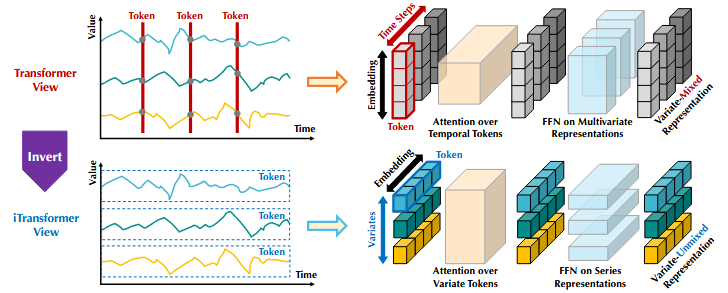
\includegraphics[width=\textwidth]{sota/iTransformer.png}
            \caption[Comparison between vanilla Transformer and iTransformer \cite{liuITransformerInvertedTransformers2023}]{Comparison between vanilla Transformer and iTransformer \cite{liuITransformerInvertedTransformers2023}}
            \label{fig::iTransformer}
 \end{figure}
 
%The gains of inverting the input is significant. In the experiments the developers of the iTransformer found, that inverting the input had a benefit for various Transformers, namely the vanilla Transformer, Reformer, Informer, Flowformer and Flashformer. 
%This research was done on weather data, traffic data and data about the hourly electricity consumption (ECL).
%For the training of the iTransformer an updated training procedure was applied. 
%For each batch only a subset of the variates are selected and the model is trained on them. 
%The updated training process is a lot fasater, while the performance is still comparable with full-variate training. 
%Another benefit of this training method is that the needed memory can be reduced significantly as shown in figure \ref{fig::iTransformer_Training} \cite{liuITransformerInvertedTransformers2023}

\begin{figure}[ht]
            \centering
            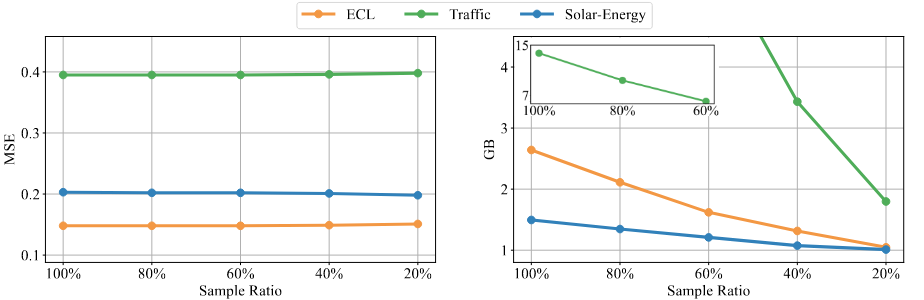
\includegraphics[width=\textwidth]{sota/iTransformer_Training.png}
            \caption[Training Performance (left) and training memory footprint (right) for training on only a subset of variates \cite{liuITransformerInvertedTransformers2023}]{Training Performance (left) and training memory footprint (right) for training on only a subset of variates \cite{liuITransformerInvertedTransformers2023}}
            \label{fig::iTransformer_Training}
 \end{figure}

\end{document}


